\section{OpAmps AC}

Der Operationsverstärker ist in allgemeiner Näherung ein Tiefpass-Filter n-ter Ordnung mit linearer Verstärkung.

 \begin{tabular}{|p{0.15\linewidth}|p{0.45\linewidth}|p{0.35\linewidth}|}
 	\hline
 	Frequenzgang allgemein
 		& \large{$A(s) = \frac{A_{0}}{(1+\frac{s}{\omega_{p_1}})(1+\frac{s}{\omega_{p_2}})\dots}$}
 		& $A_{0}=$ Lineare Verstärkung \newline $\omega{p_i}=$ Polkreisfrequenzen \\
 	\hline
 \end{tabular}
 
\subsection{Open-Loop/Closed-Loop Verhalten}

\begin{tabular}{|p{0.45\linewidth}|p{0.45\linewidth}|}
	\hline
	\textbf{Open-Loop}
		& \textbf{Closed-Loop}\\
	\hline
	\multicolumn{2}{|c|}{\textbf{Blockschemas}}\\
	\hline
	\begin{minipage}{0.4\linewidth}
	 	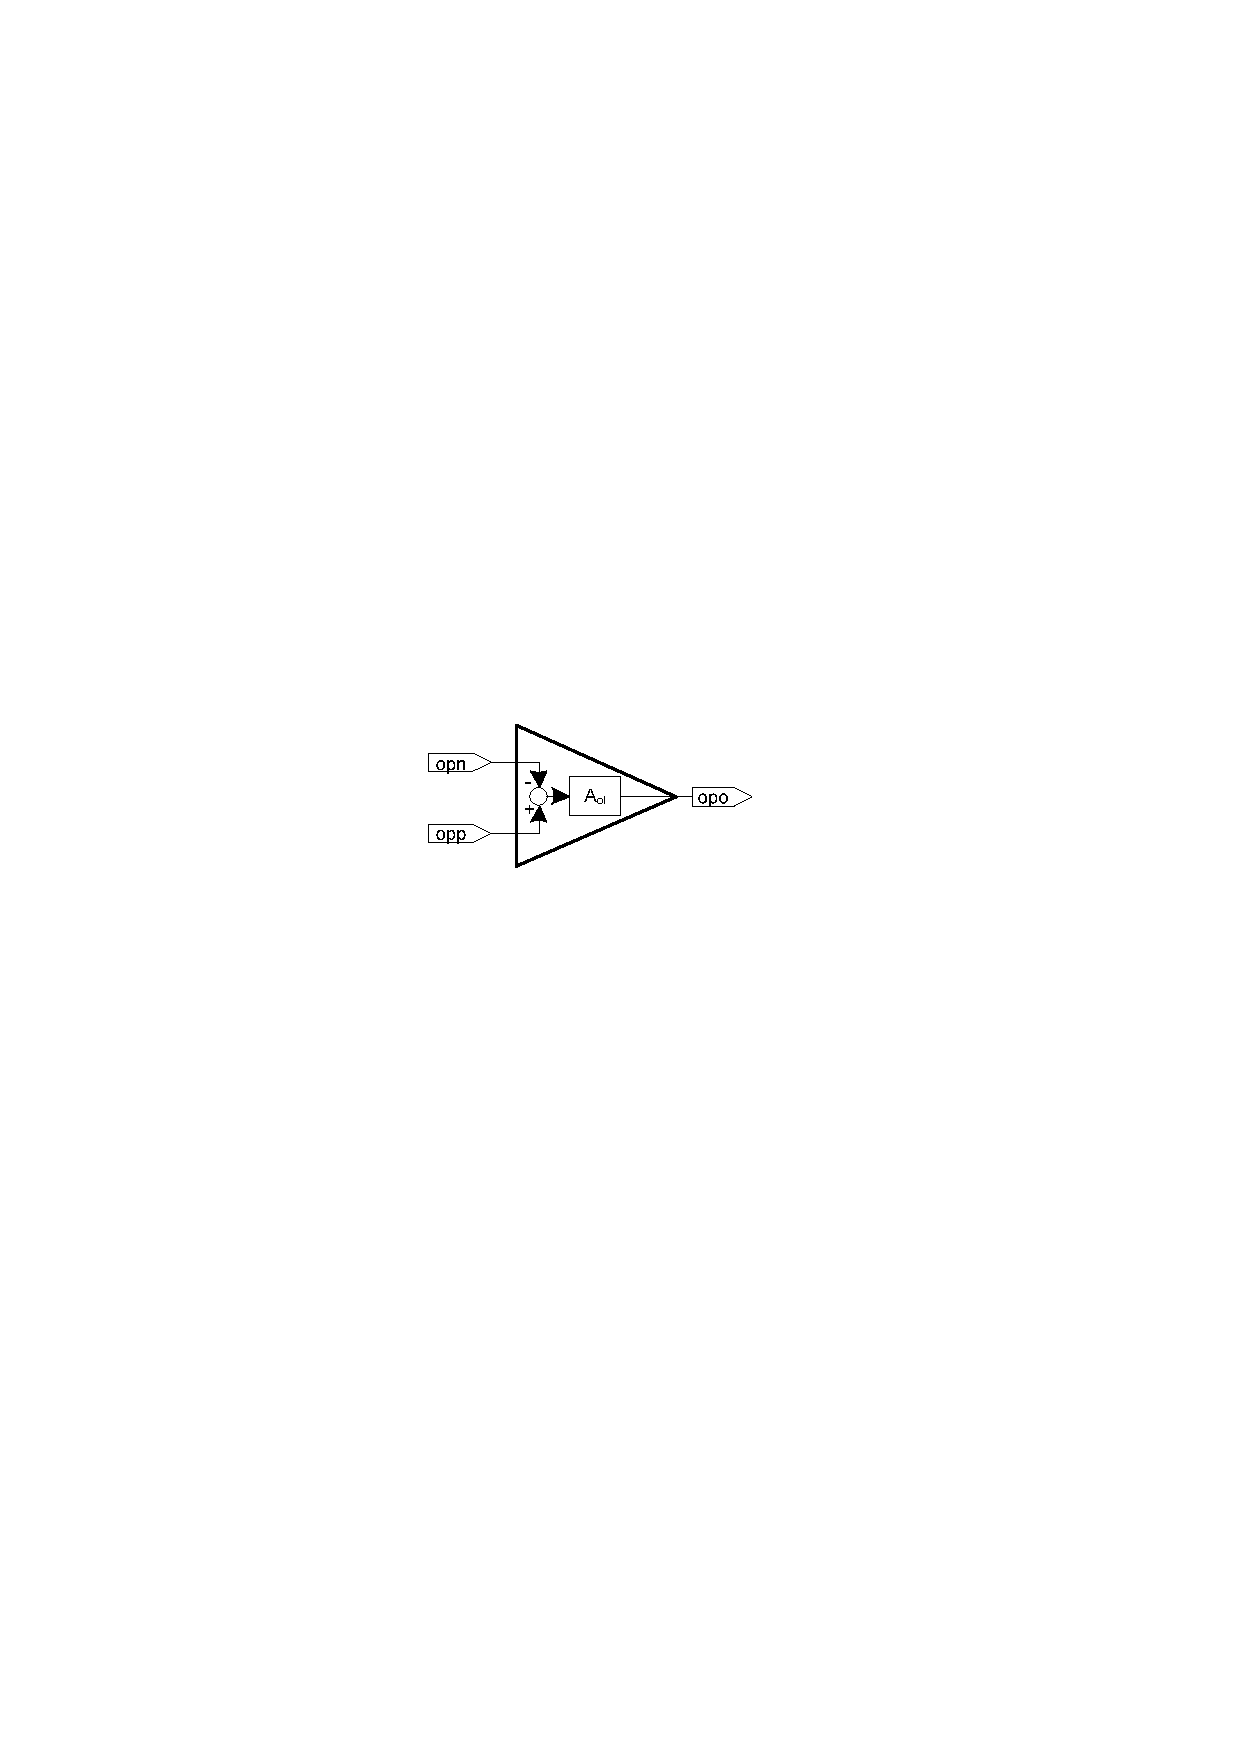
\includegraphics{./pictures/opAmpOL.pdf}
	\end{minipage}
		& \begin{minipage}{0.4\linewidth}
			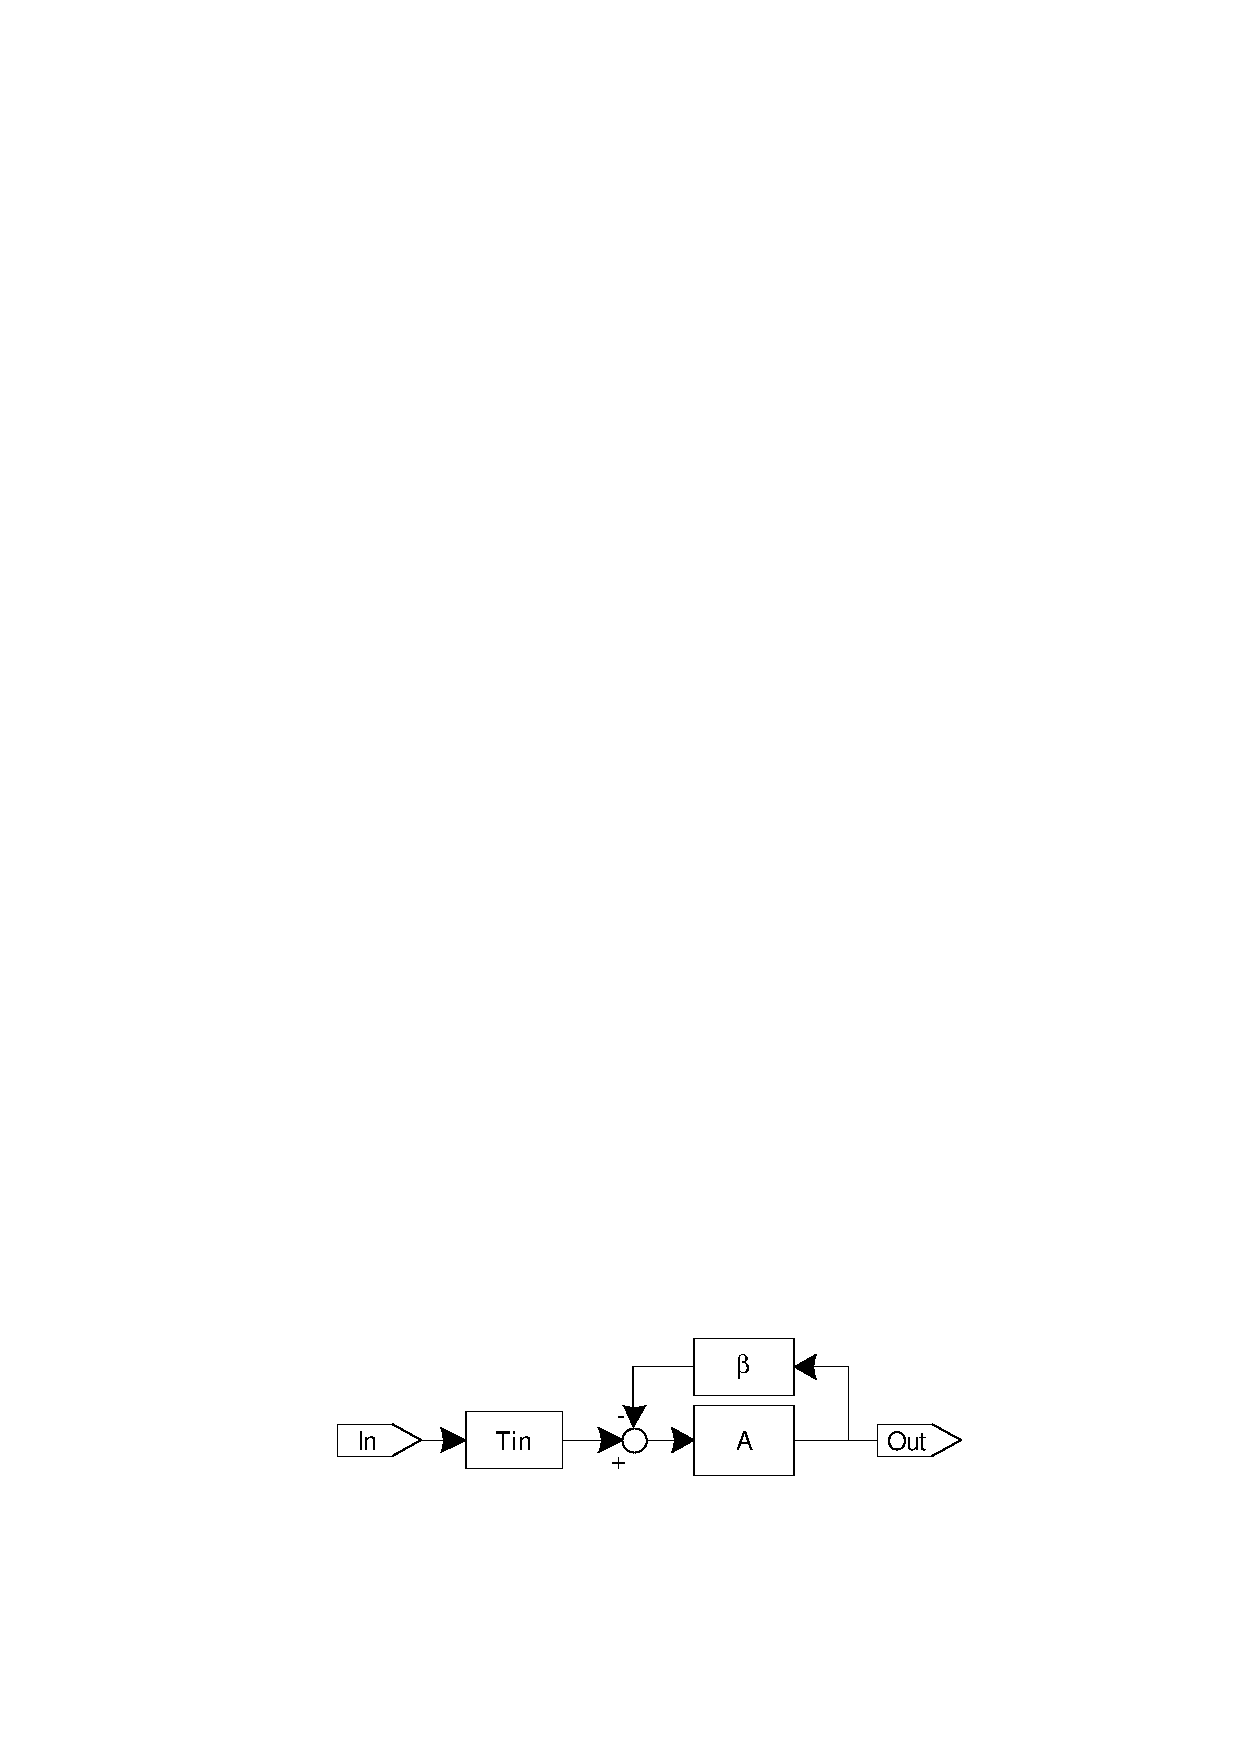
\includegraphics[height=2cm, width=8cm]{./pictures/opAmpCL.pdf}
		  \end{minipage}\\
	\hline
	\multicolumn{2}{|c|}{\textbf{Frequenzgänge}}\\
	\hline
	\large{$A_{ol}(s)=\frac{A_{ol_0}}{(1+\frac{s}{\omega_{p_{ol_1}}})(1+\frac{s}{\omega_{p_{ol_2}}})\dots}$}
		& $\begin{aligned} A_{ol}(s) &= \frac{A_{cl_0}}{(1+\frac{s}{\omega_{p_{cl_1}}})(1+\frac{s}{\omega_{p_{cl_2}}})\dots} \\
											  &= \frac{T_{in}\cdot A_{ol_0}}{1+\beta(s)\cdot A_{ol_0}}\\
									 \beta(s) &= \frac{U_{opn}}{U_{out}}\text{oder}\frac{U_{opp}}{U_{out}}\\
									 T_{in}(s) &= \frac{U_{opn}}{U_{in}}\text{oder}\frac{U_{opp}}{U_{in}}\\
								\end{aligned}$\\
	\hline
\end{tabular}

\begin{tabular}{p{0.45\linewidth}p{0.45\linewidth}}
	Durch das Schliessen des Loops wird die Bandbreite vergrössert, das gain-bandwidth-product(GBP) bleibt jedoch konstant. Die Verstärkung wird jedoch um $Tf_0(s)$ reduziert. Der Phasengang wird durch das Verschieben des ersten Poles auch verändert, wie folgende Grafik zeigt.
		& 	\begin{minipage}{0.4\linewidth}
				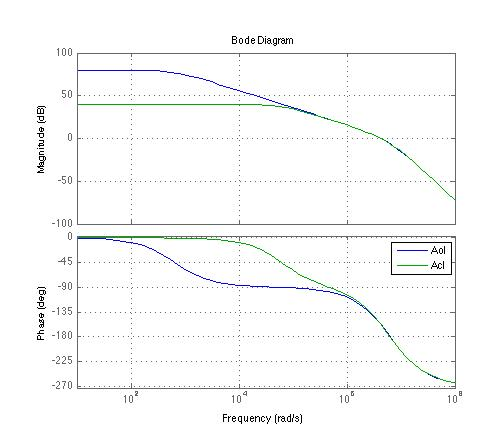
\includegraphics[height=8cm, width=10cm]{./pictures/AolAcl.jpg}
			\end{minipage}
\end{tabular}

\subsection{Stabilität des Systems}

\begin{tabular}{p{0.45\linewidth}p{0.45\linewidth}}
	Um die Stabilität des OpAmps zu betrachten, wird der Loop geöffnet. Damit das System stabil ist, darf das Fehlersignal sich selbst nicht verstärken. Damit dies der Fall ist muss der Loop gain bei einer Phase von $-180^\circ$ nicht $>1$ sein, da das Vergleichsglied die Phase noch um $180^\circ$ dreht. Ein Mass für die Stabilität ist die Phasenmarge(Phase Margin) und die Verstärkungsmarge(Gain Margin). 
	& \begin{minipage}{0.4\linewidth}
		 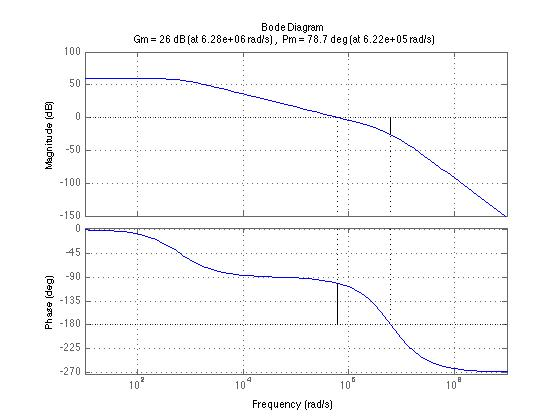
\includegraphics[height=8cm, width=10cm]{./pictures/margins.jpg}
	  \end{minipage}\\
\end{tabular}
